\documentclass{standalone}
\usepackage{tikz}

\usetikzlibrary{calc,shadows}


\begin{document}

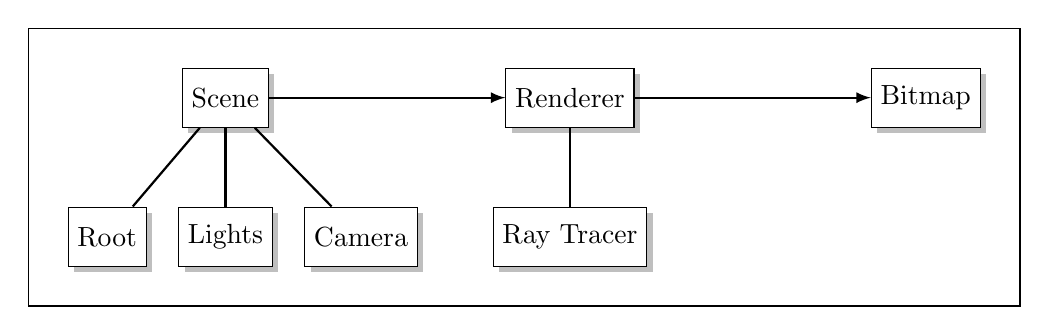
\begin{tikzpicture}[object/.style={draw,minimum height=.75cm,fill=white,drop shadow},link/.style={thick}, arrow/.style={-latex,thick}]
  \node[object] (scene) {Scene};
  \node[object,anchor=north east] (root) at ($ (scene.south) + (-1, -1) $) {Root};
  \node[object,anchor=north] (lights) at ($ (scene.south) + (0, -1) $) {Lights};
  \node[object,anchor=north west] (camera) at ($ (scene.south) + (1, -1) $) {Camera};

  \node[object,anchor=west] (renderer) at ($ (scene.east) + (3,0) $) {Renderer};
  \node[object,anchor=north] (ray tracer) at ($ (renderer.south) + (0,-1) $) {Ray Tracer};

  \node[object,anchor=west] (bitmap) at ($ (renderer.east) + (3,0) $) {Bitmap};

  \draw[link] (scene) -- (root);
  \draw[link] (scene) -- (lights);
  \draw[link] (scene) -- (camera);

  \draw[link] (renderer) -- (ray tracer);

  \draw[arrow] (scene) -- (renderer);
  \draw[arrow] (renderer) -- (bitmap);

  \draw ($ (root.south west) + (-.5, -.5) $) rectangle ($ (bitmap.north east) + (.5, .5) $);
\end{tikzpicture}

\end{document}